% Created 2024-04-17 Wed 19:40
% Intended LaTeX compiler: xelatex
\documentclass[11pt]{article}
\usepackage{hyperref}
% wrong resolution of image
% https://tex.stackexchange.com/questions/21627/image-from-includegraphics-showing-in-wrong-image-size?rq=1

%%%%%%%%%%%%%%%%%%%%%%%%%%%%%%%%%%%%%%
%% TIPS                                 %%
%%%%%%%%%%%%%%%%%%%%%%%%%%%%%%%%%%%%%%
% \substack{a\\b} for multiple lines text
% \usepackage{expl3}
% \expandafter\def\csname ver@l3regex.sty\endcsname{}
% \usepackage{pkgloader}
\usepackage[utf8]{inputenc}

% nfss error
% \usepackage[B1,T1]{fontenc}
\usepackage{fontspec}

% \usepackage[Emoticons]{ucharclasses}
\newfontfamily\DejaSans{DejaVu Sans}
% \setDefaultTransitions{\DejaSans}{}

% pdfplots will load xolor automatically without option
\usepackage[dvipsnames]{xcolor}

%                                                             ┳┳┓   ┓
%                                                             ┃┃┃┏┓╋┣┓
%                                                             ┛ ┗┗┻┗┛┗
% \usepackage{amsmath} mathtools loads the amsmath
\usepackage{amsmath}
\usepackage{mathtools}

\usepackage{amsthm}
\usepackage{amsbsy}

%\usepackage{commath}

\usepackage{amssymb}

\usepackage{mathrsfs}
%\usepackage{mathabx}
\usepackage{stmaryrd}
\usepackage{empheq}

\usepackage{scalerel}
\usepackage{stackengine}
\usepackage{stackrel}



\usepackage{nicematrix}
\usepackage{tensor}
\usepackage{blkarray}
\usepackage{siunitx}
\usepackage[f]{esvect}

% centering \not on a letter
\usepackage{slashed}
\usepackage[makeroom]{cancel}

%\usepackage{merriweather}
\usepackage{unicode-math}
\setmainfont{TeX Gyre Pagella}
% \setmathfont{STIX}
%\setmathfont{texgyrepagella-math.otf}
%\setmathfont{Libertinus Math}
\setmathfont{Latin Modern Math}

 % \setmathfont[range={\smwhtdiamond,\enclosediamond,\varlrtriangle}]{Latin Modern Math}
\setmathfont[range={\rightrightarrows,\twoheadrightarrow,\leftrightsquigarrow,\triangledown,\vartriangle,\precneq,\succneq,\prec,\succ,\preceq,\succeq,\tieconcat}]{XITS Math}
 \setmathfont[range={\int,\setminus}]{Libertinus Math}
 % \setmathfont[range={\mathalpha}]{TeX Gyre Pagella Math}
%\setmathfont[range={\mitA,\mitB,\mitC,\mitD,\mitE,\mitF,\mitG,\mitH,\mitI,\mitJ,\mitK,\mitL,\mitM,\mitN,\mitO,\mitP,\mitQ,\mitR,\mitS,\mitT,\mitU,\mitV,\mitW,\mitX,\mitY,\mitZ,\mita,\mitb,\mitc,\mitd,\mite,\mitf,\mitg,\miti,\mitj,\mitk,\mitl,\mitm,\mitn,\mito,\mitp,\mitq,\mitr,\mits,\mitt,\mitu,\mitv,\mitw,\mitx,\mity,\mitz}]{TeX Gyre Pagella Math}
% unicode is not good at this!
%\let\nmodels\nvDash

 \usepackage{wasysym}

 % for wide hat
 \DeclareSymbolFont{yhlargesymbols}{OMX}{yhex}{m}{n} \DeclareMathAccent{\what}{\mathord}{yhlargesymbols}{"62}

%                                                               ┏┳┓•┓
%                                                                ┃ ┓┃┏┓
%                                                                ┻ ┗┛┗┗

\usepackage{pgfplots}
\pgfplotsset{compat=1.18}
\usepackage{tikz}
\usepackage{tikz-cd}
\tikzcdset{scale cd/.style={every label/.append style={scale=#1},
    cells={nodes={scale=#1}}}}
% TODO: discard qtree and use forest
% \usepackage{tikz-qtree}
\usepackage{forest}

\usetikzlibrary{arrows,positioning,calc,fadings,decorations,matrix,decorations,shapes.misc}
%setting from geogebra
\definecolor{ccqqqq}{rgb}{0.8,0,0}

%                                                          ┳┳┓•    ┓┓
%                                                          ┃┃┃┓┏┏┏┓┃┃┏┓┏┓┏┓┏┓┓┏┏
%                                                          ┛ ┗┗┛┗┗ ┗┗┗┻┛┗┗ ┗┛┗┻┛
%\usepackage{twemojis}
\usepackage[most]{tcolorbox}
\usepackage{threeparttable}
\usepackage{tabularx}

\usepackage{enumitem}
\usepackage[indLines=false]{algpseudocodex}
\usepackage[]{algorithm2e}
% \SetKwComment{Comment}{/* }{ */}
% \algrenewcommand\algorithmicrequire{\textbf{Input:}}
% \algrenewcommand\algorithmicensure{\textbf{Output:}}
% wrong with preview
\usepackage{subcaption}
\usepackage{caption}
% {\aunclfamily\Huge}
\usepackage{auncial}

\usepackage{float}

\usepackage{fancyhdr}

\usepackage{ifthen}
\usepackage{xargs}

\definecolor{mintedbg}{rgb}{0.99,0.99,0.99}
\usepackage[cachedir=\detokenize{~/miscellaneous/trash}]{minted}
\setminted{breaklines,
  mathescape,
  bgcolor=mintedbg,
  fontsize=\footnotesize,
  frame=single,
  linenos}
\usemintedstyle{xcode}
\usepackage{tcolorbox}
\usepackage{etoolbox}



\usepackage{imakeidx}
\usepackage{hyperref}
\usepackage{soul}
\usepackage{framed}

% don't use this for preview
%\usepackage[margin=1.5in]{geometry}
% \usepackage{geometry}
% \geometry{legalpaper, landscape, margin=1in}
\usepackage[font=itshape]{quoting}

%\LoadPackagesNow
%\usepackage[xetex]{preview}
%%%%%%%%%%%%%%%%%%%%%%%%%%%%%%%%%%%%%%%
%% USEPACKAGES end                       %%
%%%%%%%%%%%%%%%%%%%%%%%%%%%%%%%%%%%%%%%

%%%%%%%%%%%%%%%%%%%%%%%%%%%%%%%%%%%%%%%
%% Algorithm environment
%%%%%%%%%%%%%%%%%%%%%%%%%%%%%%%%%%%%%%%
\SetKwIF{Recv}{}{}{upon receiving}{do}{}{}{}
\SetKwBlock{Init}{initially do}{}
\SetKwProg{Function}{Function}{:}{}

% https://github.com/chrmatt/algpseudocodex/issues/3
\algnewcommand\algorithmicswitch{\textbf{switch}}%
\algnewcommand\algorithmiccase{\textbf{case}}
\algnewcommand\algorithmicof{\textbf{of}}
\algnewcommand\algorithmicotherwise{\texttt{otherwise} $\Rightarrow$}

\makeatletter
\algdef{SE}[SWITCH]{Switch}{EndSwitch}[1]{\algpx@startIndent\algpx@startCodeCommand\algorithmicswitch\ #1\ \algorithmicdo}{\algpx@endIndent\algpx@startCodeCommand\algorithmicend\ \algorithmicswitch}%
\algdef{SE}[CASE]{Case}{EndCase}[1]{\algpx@startIndent\algpx@startCodeCommand\algorithmiccase\ #1}{\algpx@endIndent\algpx@startCodeCommand\algorithmicend\ \algorithmiccase}%
\algdef{SE}[CASEOF]{CaseOf}{EndCaseOf}[1]{\algpx@startIndent\algpx@startCodeCommand\algorithmiccase\ #1 \algorithmicof}{\algpx@endIndent\algpx@startCodeCommand\algorithmicend\ \algorithmiccase}
\algdef{SE}[OTHERWISE]{Otherwise}{EndOtherwise}[0]{\algpx@startIndent\algpx@startCodeCommand\algorithmicotherwise}{\algpx@endIndent\algpx@startCodeCommand\algorithmicend\ \algorithmicotherwise}
\ifbool{algpx@noEnd}{%
  \algtext*{EndSwitch}%
  \algtext*{EndCase}%
  \algtext*{EndCaseOf}
  \algtext*{EndOtherwise}
  %
  % end indent line after (not before), to get correct y position for multiline text in last command
  \apptocmd{\EndSwitch}{\algpx@endIndent}{}{}%
  \apptocmd{\EndCase}{\algpx@endIndent}{}{}%
  \apptocmd{\EndCaseOf}{\algpx@endIndent}{}{}
  \apptocmd{\EndOtherwise}{\algpx@endIndent}{}{}
}{}%

\pretocmd{\Switch}{\algpx@endCodeCommand}{}{}
\pretocmd{\Case}{\algpx@endCodeCommand}{}{}
\pretocmd{\CaseOf}{\algpx@endCodeCommand}{}{}
\pretocmd{\Otherwise}{\algpx@endCodeCommand}{}{}

% for end commands that may not be printed, tell endCodeCommand whether we are using noEnd
\ifbool{algpx@noEnd}{%
  \pretocmd{\EndSwitch}{\algpx@endCodeCommand[1]}{}{}%
  \pretocmd{\EndCase}{\algpx@endCodeCommand[1]}{}{}
  \pretocmd{\EndCaseOf}{\algpx@endCodeCommand[1]}{}{}%
  \pretocmd{\EndOtherwise}{\algpx@endCodeCommand[1]}{}{}
}{%
  \pretocmd{\EndSwitch}{\algpx@endCodeCommand[0]}{}{}%
  \pretocmd{\EndCase}{\algpx@endCodeCommand[0]}{}{}%
  \pretocmd{\EndCaseOf}{\algpx@endCodeCommand[0]}{}{}
  \pretocmd{\EndOtherwise}{\algpx@endCodeCommand[0]}{}{}
}%
\makeatother
% % For algpseudocode
% \algnewcommand\algorithmicswitch{\textbf{switch}}
% \algnewcommand\algorithmiccase{\textbf{case}}
% \algnewcommand\algorithmiccaseof{\textbf{case}}
% \algnewcommand\algorithmicof{\textbf{of}}
% % New "environments"
% \algdef{SE}[SWITCH]{Switch}{EndSwitch}[1]{\algorithmicswitch\ #1\ \algorithmicdo}{\algorithmicend\ \algorithmicswitch}%
% \algdef{SE}[CASE]{Case}{EndCase}[1]{\algorithmiccase\ #1}{\algorithmicend\ \algorithmiccase}%
% \algtext*{EndSwitch}%
% \algtext*{EndCase}
% \algdef{SE}[CASEOF]{CaseOf}{EndCaseOf}[1]{\algorithmiccaseof\ #1 \algorithmicof}{\algorithmicend\ \algorithmiccaseof}
% \algtext*{EndCaseOf}



%\pdfcompresslevel0

% quoting from
% https://tex.stackexchange.com/questions/391726/the-quotation-environment
\NewDocumentCommand{\bywhom}{m}{% the Bourbaki trick
  {\nobreak\hfill\penalty50\hskip1em\null\nobreak
   \hfill\mbox{\normalfont(#1)}%
   \parfillskip=0pt \finalhyphendemerits=0 \par}%
}

\NewDocumentEnvironment{pquotation}{m}
  {\begin{quoting}[
     indentfirst=true,
     leftmargin=\parindent,
     rightmargin=\parindent]\itshape}
  {\bywhom{#1}\end{quoting}}

\indexsetup{othercode=\small}
\makeindex[columns=2,options={-s /media/wu/file/stuuudy/notes/index_style.ist},intoc]
\makeatletter
\def\@idxitem{\par\hangindent 0pt}
\makeatother


% \newcounter{dummy} \numberwithin{dummy}{section}
\newtheorem{dummy}{dummy}[section]
\theoremstyle{definition}
\newtheorem{definition}[dummy]{Definition}
\theoremstyle{plain}
\newtheorem{corollary}[dummy]{Corollary}
\newtheorem{lemma}[dummy]{Lemma}
\newtheorem{proposition}[dummy]{Proposition}
\newtheorem{theorem}[dummy]{Theorem}
\newtheorem{notation}[dummy]{Notation}
\newtheorem{conjecture}[dummy]{Conjecture}
\newtheorem{fact}[dummy]{Fact}
\newtheorem{warning}[dummy]{Warning}
\theoremstyle{definition}
\newtheorem{examplle}{Example}[section]
\theoremstyle{remark}
\newtheorem*{remark}{Remark}
\newtheorem{exercise}{Exercise}[subsection]
\newtheorem{problem}{Problem}[subsection]
\newtheorem{observation}{Observation}[section]
\newenvironment{claim}[1]{\par\noindent\textbf{Claim:}\space#1}{}

\makeatletter
\DeclareFontFamily{U}{tipa}{}
\DeclareFontShape{U}{tipa}{m}{n}{<->tipa10}{}
\newcommand{\arc@char}{{\usefont{U}{tipa}{m}{n}\symbol{62}}}%

\newcommand{\arc}[1]{\mathpalette\arc@arc{#1}}

\newcommand{\arc@arc}[2]{%
  \sbox0{$\m@th#1#2$}%
  \vbox{
    \hbox{\resizebox{\wd0}{\height}{\arc@char}}
    \nointerlineskip
    \box0
  }%
}
\makeatother

\setcounter{MaxMatrixCols}{20}
%%%%%%% ABS
\DeclarePairedDelimiter\abss{\lvert}{\rvert}%
\DeclarePairedDelimiter\normm{\lVert}{\rVert}%

% Swap the definition of \abs* and \norm*, so that \abs
% and \norm resizes the size of the brackets, and the
% starred version does not.
\makeatletter
\let\oldabs\abss
%\def\abs{\@ifstar{\oldabs}{\oldabs*}}
\newcommand{\abs}{\@ifstar{\oldabs}{\oldabs*}}
\newcommand{\norm}[1]{\left\lVert#1\right\rVert}
%\let\oldnorm\normm
%\def\norm{\@ifstar{\oldnorm}{\oldnorm*}}
%\renewcommand{norm}{\@ifstar{\oldnorm}{\oldnorm*}}
\makeatother

% \stackMath
% \newcommand\what[1]{%
% \savestack{\tmpbox}{\stretchto{%
%   \scaleto{%
%     \scalerel*[\widthof{\ensuremath{#1}}]{\kern-.6pt\bigwedge\kern-.6pt}%
%     {\rule[-\textheight/2]{1ex}{\textheight}}%WIDTH-LIMITED BIG WEDGE
%   }{\textheight}%
% }{0.5ex}}%
% \stackon[1pt]{#1}{\tmpbox}%
% }

% \newcommand\what[1]{\ThisStyle{%
%     \setbox0=\hbox{$\SavedStyle#1$}%
%     \stackengine{-1.0\ht0+.5pt}{$\SavedStyle#1$}{%
%       \stretchto{\scaleto{\SavedStyle\mkern.15mu\char'136}{2.6\wd0}}{1.4\ht0}%
%     }{O}{c}{F}{T}{S}%
%   }
% }

% \newcommand\wtilde[1]{\ThisStyle{%
%     \setbox0=\hbox{$\SavedStyle#1$}%
%     \stackengine{-.1\LMpt}{$\SavedStyle#1$}{%
%       \stretchto{\scaleto{\SavedStyle\mkern.2mu\AC}{.5150\wd0}}{.6\ht0}%
%     }{O}{c}{F}{T}{S}%
%   }
% }

% \newcommand\wbar[1]{\ThisStyle{%
%     \setbox0=\hbox{$\SavedStyle#1$}%
%     \stackengine{.5pt+\LMpt}{$\SavedStyle#1$}{%
%       \rule{\wd0}{\dimexpr.3\LMpt+.3pt}%
%     }{O}{c}{F}{T}{S}%
%   }
% }

\newcommand{\bl}[1] {\boldsymbol{#1}}
\newcommand{\Wt}[1] {\stackrel{\sim}{\smash{#1}\rule{0pt}{1.1ex}}}
\newcommand{\wt}[1] {\widetilde{#1}}
\newcommand{\tf}[1] {\textbf{#1}}

\newcommand{\wu}[1]{{\color{red} #1}}

%For boxed texts in align, use Aboxed{}
%otherwise use boxed{}

\DeclareMathSymbol{\widehatsym}{\mathord}{largesymbols}{"62}
\newcommand\lowerwidehatsym{%
  \text{\smash{\raisebox{-1.3ex}{%
    $\widehatsym$}}}}
\newcommand\fixwidehat[1]{%
  \mathchoice
    {\accentset{\displaystyle\lowerwidehatsym}{#1}}
    {\accentset{\textstyle\lowerwidehatsym}{#1}}
    {\accentset{\scriptstyle\lowerwidehatsym}{#1}}
    {\accentset{\scriptscriptstyle\lowerwidehatsym}{#1}}
  }


\newcommand{\cupdot}{\mathbin{\dot{\cup}}}
\newcommand{\bigcupdot}{\mathop{\dot{\bigcup}}}

\usepackage{graphicx}

\usepackage[toc,page]{appendix}

% text on arrow for xRightarrow
\makeatletter
%\newcommand{\xRightarrow}[2][]{\ext@arrow 0359\Rightarrowfill@{#1}{#2}}
\makeatother

% Arbitrary long arrow
\newcommand{\Rarrow}[1]{%
\parbox{#1}{\tikz{\draw[->](0,0)--(#1,0);}}
}

\newcommand{\LRarrow}[1]{%
\parbox{#1}{\tikz{\draw[<->](0,0)--(#1,0);}}
}


\makeatletter
\providecommand*{\rmodels}{%
  \mathrel{%
    \mathpalette\@rmodels\models
  }%
}
\newcommand*{\@rmodels}[2]{%
  \reflectbox{$\m@th#1#2$}%
}
\makeatother

% Roman numerals
\makeatletter
\newcommand*{\rom}[1]{\expandafter\@slowromancap\romannumeral #1@}
\makeatother
% \\def \\b\([a-zA-Z]\) {\\boldsymbol{[a-zA-z]}}
% \\DeclareMathOperator{\\b\1}{\\textbf{\1}}

\DeclareMathOperator*{\argmin}{arg\,min}
\DeclareMathOperator*{\argmax}{arg\,max}

\DeclareMathOperator{\bone}{\textbf{1}}
\DeclareMathOperator{\bx}{\textbf{x}}
\DeclareMathOperator{\bz}{\textbf{z}}
\DeclareMathOperator{\bff}{\textbf{f}}
\DeclareMathOperator{\ba}{\textbf{a}}
\DeclareMathOperator{\bk}{\textbf{k}}
\DeclareMathOperator{\bs}{\textbf{s}}
\DeclareMathOperator{\bh}{\textbf{h}}
\DeclareMathOperator{\bc}{\textbf{c}}
\DeclareMathOperator{\br}{\textbf{r}}
\DeclareMathOperator{\bi}{\textbf{i}}
\DeclareMathOperator{\bj}{\textbf{j}}
\DeclareMathOperator{\bn}{\textbf{n}}
\DeclareMathOperator{\be}{\textbf{e}}
\DeclareMathOperator{\bo}{\textbf{o}}
\DeclareMathOperator{\bU}{\textbf{U}}
\DeclareMathOperator{\bL}{\textbf{L}}
\DeclareMathOperator{\bV}{\textbf{V}}
\def \bzero {\mathbf{0}}
\def \bbone {\mathbb{1}}
\def \btwo {\mathbf{2}}
\DeclareMathOperator{\bv}{\textbf{v}}
\DeclareMathOperator{\bp}{\textbf{p}}
\DeclareMathOperator{\bI}{\textbf{I}}
\def \dbI {\dot{\bI}}
\DeclareMathOperator{\bM}{\textbf{M}}
\DeclareMathOperator{\bN}{\textbf{N}}
\DeclareMathOperator{\bK}{\textbf{K}}
\DeclareMathOperator{\bt}{\textbf{t}}
\DeclareMathOperator{\bb}{\textbf{b}}
\DeclareMathOperator{\bA}{\textbf{A}}
\DeclareMathOperator{\bX}{\textbf{X}}
\DeclareMathOperator{\bu}{\textbf{u}}
\DeclareMathOperator{\bS}{\textbf{S}}
\DeclareMathOperator{\bZ}{\textbf{Z}}
\DeclareMathOperator{\bJ}{\textbf{J}}
\DeclareMathOperator{\by}{\textbf{y}}
\DeclareMathOperator{\bw}{\textbf{w}}
\DeclareMathOperator{\bT}{\textbf{T}}
\DeclareMathOperator{\bF}{\textbf{F}}
\DeclareMathOperator{\bmm}{\textbf{m}}
\DeclareMathOperator{\bW}{\textbf{W}}
\DeclareMathOperator{\bR}{\textbf{R}}
\DeclareMathOperator{\bC}{\textbf{C}}
\DeclareMathOperator{\bD}{\textbf{D}}
\DeclareMathOperator{\bE}{\textbf{E}}
\DeclareMathOperator{\bQ}{\textbf{Q}}
\DeclareMathOperator{\bP}{\textbf{P}}
\DeclareMathOperator{\bY}{\textbf{Y}}
\DeclareMathOperator{\bH}{\textbf{H}}
\DeclareMathOperator{\bB}{\textbf{B}}
\DeclareMathOperator{\bG}{\textbf{G}}
\def \blambda {\symbf{\lambda}}
\def \boldeta {\symbf{\eta}}
\def \balpha {\symbf{\alpha}}
\def \btau {\symbf{\tau}}
\def \bbeta {\symbf{\beta}}
\def \bgamma {\symbf{\gamma}}
\def \bxi {\symbf{\xi}}
\def \bLambda {\symbf{\Lambda}}
\def \bGamma {\symbf{\Gamma}}

\newcommand{\bto}{{\boldsymbol{\to}}}
\newcommand{\Ra}{\Rightarrow}
\newcommand{\xrsa}[1]{\overset{#1}{\rightsquigarrow}}
\newcommand{\xlsa}[1]{\overset{#1}{\leftsquigarrow}}
\newcommand\und[1]{\underline{#1}}
\newcommand\ove[1]{\overline{#1}}
%\def \concat {\verb|^|}
\def \bPhi {\mbfPhi}
\def \btheta {\mbftheta}
\def \bTheta {\mbfTheta}
\def \bmu {\mbfmu}
\def \bphi {\mbfphi}
\def \bSigma {\mbfSigma}
\def \la {\langle}
\def \ra {\rangle}

\def \caln {\mathcal{N}}
\def \dissum {\displaystyle\Sigma}
\def \dispro {\displaystyle\prod}

\def \caret {\verb!^!}

\def \A {\mathbb{A}}
\def \B {\mathbb{B}}
\def \C {\mathbb{C}}
\def \D {\mathbb{D}}
\def \E {\mathbb{E}}
\def \F {\mathbb{F}}
\def \G {\mathbb{G}}
\def \H {\mathbb{H}}
\def \I {\mathbb{I}}
\def \J {\mathbb{J}}
\def \K {\mathbb{K}}
\def \L {\mathbb{L}}
\def \M {\mathbb{M}}
\def \N {\mathbb{N}}
\def \O {\mathbb{O}}
\def \P {\mathbb{P}}
\def \Q {\mathbb{Q}}
\def \R {\mathbb{R}}
\def \S {\mathbb{S}}
\def \T {\mathbb{T}}
\def \U {\mathbb{U}}
\def \V {\mathbb{V}}
\def \W {\mathbb{W}}
\def \X {\mathbb{X}}
\def \Y {\mathbb{Y}}
\def \Z {\mathbb{Z}}

\def \cala {\mathcal{A}}
\def \cale {\mathcal{E}}
\def \calb {\mathcal{B}}
\def \calq {\mathcal{Q}}
\def \calp {\mathcal{P}}
\def \cals {\mathcal{S}}
\def \calx {\mathcal{X}}
\def \caly {\mathcal{Y}}
\def \calg {\mathcal{G}}
\def \cald {\mathcal{D}}
\def \caln {\mathcal{N}}
\def \calr {\mathcal{R}}
\def \calt {\mathcal{T}}
\def \calm {\mathcal{M}}
\def \calw {\mathcal{W}}
\def \calc {\mathcal{C}}
\def \calv {\mathcal{V}}
\def \calf {\mathcal{F}}
\def \calk {\mathcal{K}}
\def \call {\mathcal{L}}
\def \calu {\mathcal{U}}
\def \calo {\mathcal{O}}
\def \calh {\mathcal{H}}
\def \cali {\mathcal{I}}
\def \calj {\mathcal{J}}

\def \bcup {\bigcup}

% set theory

\def \zfcc {\textbf{ZFC}^-}
\def \BGC {\textbf{BGC}}
\def \BG {\textbf{BG}}
\def \ac  {\textbf{AC}}
\def \gl  {\textbf{L }}
\def \gll {\textbf{L}}
\newcommand{\zfm}{$\textbf{ZF}^-$}

\def \ZFm {\text{ZF}^-}
\def \ZFCm {\text{ZFC}^-}
\DeclareMathOperator{\WF}{WF}
\DeclareMathOperator{\On}{On}
\def \on {\textbf{On }}
\def \cm {\textbf{M }}
\def \cn {\textbf{N }}
\def \cv {\textbf{V }}
\def \zc {\textbf{ZC }}
\def \zcm {\textbf{ZC}}
\def \zff {\textbf{ZF}}
\def \wfm {\textbf{WF}}
\def \onm {\textbf{On}}
\def \cmm {\textbf{M}}
\def \cnm {\textbf{N}}
\def \cvm {\textbf{V}}

\renewcommand{\restriction}{\mathord{\upharpoonright}}
%% another restriction
\newcommand\restr[2]{{% we make the whole thing an ordinary symbol
  \left.\kern-\nulldelimiterspace % automatically resize the bar with \right
  #1 % the function
  \vphantom{\big|} % pretend it's a little taller at normal size
  \right|_{#2} % this is the delimiter
  }}

\def \pred {\text{pred}}

\def \rank {\text{rank}}
\def \Con {\text{Con}}
\def \deff {\text{Def}}


\def \uin {\underline{\in}}
\def \oin {\overline{\in}}
\def \uR {\underline{R}}
\def \oR {\overline{R}}
\def \uP {\underline{P}}
\def \oP {\overline{P}}

\def \dsum {\displaystyle\sum}

\def \Ra {\Rightarrow}

\def \e {\enspace}

\def \sgn {\operatorname{sgn}}
\def \gen {\operatorname{gen}}
\def \Hom {\operatorname{Hom}}
\def \hom {\operatorname{hom}}
\def \Sub {\operatorname{Sub}}

\def \supp {\operatorname{supp}}

\def \epiarrow {\twoheadarrow}
\def \monoarrow {\rightarrowtail}
\def \rrarrow {\rightrightarrows}

% \def \minus {\text{-}}
% \newcommand{\minus}{\scalebox{0.75}[1.0]{$-$}}
% \DeclareUnicodeCharacter{002D}{\minus}


\def \tril {\triangleleft}

\def \ISigma {\text{I}\Sigma}
\def \IDelta {\text{I}\Delta}
\def \IPi {\text{I}\Pi}
\def \ACF {\textsf{ACF}}
\def \pCF {\textit{p}\text{CF}}
\def \ACVF {\textsf{ACVF}}
\def \HLR {\textsf{HLR}}
\def \OAG {\textsf{OAG}}
\def \RCF {\textsf{RCF}}
\DeclareMathOperator{\GL}{GL}
\DeclareMathOperator{\PGL}{PGL}
\DeclareMathOperator{\SL}{SL}
\DeclareMathOperator{\Inv}{Inv}
\DeclareMathOperator{\res}{res}
\DeclareMathOperator{\Sym}{Sym}
%\DeclareMathOperator{\char}{char}
\def \equal {=}

\def \degree {\text{degree}}
\def \app {\text{App}}
\def \FV {\text{FV}}
\def \conv {\text{conv}}
\def \cont {\text{cont}}
\DeclareMathOperator{\cl}{\text{cl}}
\DeclareMathOperator{\trcl}{\text{trcl}}
\DeclareMathOperator{\sg}{sg}
\DeclareMathOperator{\trdeg}{trdeg}
\def \Ord {\text{Ord}}

\DeclareMathOperator{\cf}{cf}
\DeclareMathOperator{\zfc}{ZFC}

%\DeclareMathOperator{\Th}{Th}
%\def \th {\text{Th}}
% \newcommand{\th}{\text{Th}}
\DeclareMathOperator{\type}{type}
\DeclareMathOperator{\zf}{\textbf{ZF}}
\def \fa {\mathfrak{a}}
\def \fb {\mathfrak{b}}
\def \fc {\mathfrak{c}}
\def \fd {\mathfrak{d}}
\def \fe {\mathfrak{e}}
\def \ff {\mathfrak{f}}
\def \fg {\mathfrak{g}}
\def \fh {\mathfrak{h}}
%\def \fi {\mathfrak{i}}
\def \fj {\mathfrak{j}}
\def \fk {\mathfrak{k}}
\def \fl {\mathfrak{l}}
\def \fm {\mathfrak{m}}
\def \fn {\mathfrak{n}}
\def \fo {\mathfrak{o}}
\def \fp {\mathfrak{p}}
\def \fq {\mathfrak{q}}
\def \fr {\mathfrak{r}}
\def \fs {\mathfrak{s}}
\def \ft {\mathfrak{t}}
\def \fu {\mathfrak{u}}
\def \fv {\mathfrak{v}}
\def \fw {\mathfrak{w}}
\def \fx {\mathfrak{x}}
\def \fy {\mathfrak{y}}
\def \fz {\mathfrak{z}}
\def \fA {\mathfrak{A}}
\def \fB {\mathfrak{B}}
\def \fC {\mathfrak{C}}
\def \fD {\mathfrak{D}}
\def \fE {\mathfrak{E}}
\def \fF {\mathfrak{F}}
\def \fG {\mathfrak{G}}
\def \fH {\mathfrak{H}}
\def \fI {\mathfrak{I}}
\def \fJ {\mathfrak{J}}
\def \fK {\mathfrak{K}}
\def \fL {\mathfrak{L}}
\def \fM {\mathfrak{M}}
\def \fN {\mathfrak{N}}
\def \fO {\mathfrak{O}}
\def \fP {\mathfrak{P}}
\def \fQ {\mathfrak{Q}}
\def \fR {\mathfrak{R}}
\def \fS {\mathfrak{S}}
\def \fT {\mathfrak{T}}
\def \fU {\mathfrak{U}}
\def \fV {\mathfrak{V}}
\def \fW {\mathfrak{W}}
\def \fX {\mathfrak{X}}
\def \fY {\mathfrak{Y}}
\def \fZ {\mathfrak{Z}}

\def \sfA {\textsf{A}}
\def \sfB {\textsf{B}}
\def \sfC {\textsf{C}}
\def \sfD {\textsf{D}}
\def \sfE {\textsf{E}}
\def \sfF {\textsf{F}}
\def \sfG {\textsf{G}}
\def \sfH {\textsf{H}}
\def \sfI {\textsf{I}}
\def \sfJ {\textsf{J}}
\def \sfK {\textsf{K}}
\def \sfL {\textsf{L}}
\def \sfM {\textsf{M}}
\def \sfN {\textsf{N}}
\def \sfO {\textsf{O}}
\def \sfP {\textsf{P}}
\def \sfQ {\textsf{Q}}
\def \sfR {\textsf{R}}
\def \sfS {\textsf{S}}
\def \sfT {\textsf{T}}
\def \sfU {\textsf{U}}
\def \sfV {\textsf{V}}
\def \sfW {\textsf{W}}
\def \sfX {\textsf{X}}
\def \sfY {\textsf{Y}}
\def \sfZ {\textsf{Z}}
\def \sfa {\textsf{a}}
\def \sfb {\textsf{b}}
\def \sfc {\textsf{c}}
\def \sfd {\textsf{d}}
\def \sfe {\textsf{e}}
\def \sff {\textsf{f}}
\def \sfg {\textsf{g}}
\def \sfh {\textsf{h}}
\def \sfi {\textsf{i}}
\def \sfj {\textsf{j}}
\def \sfk {\textsf{k}}
\def \sfl {\textsf{l}}
\def \sfm {\textsf{m}}
\def \sfn {\textsf{n}}
\def \sfo {\textsf{o}}
\def \sfp {\textsf{p}}
\def \sfq {\textsf{q}}
\def \sfr {\textsf{r}}
\def \sfs {\textsf{s}}
\def \sft {\textsf{t}}
\def \sfu {\textsf{u}}
\def \sfv {\textsf{v}}
\def \sfw {\textsf{w}}
\def \sfx {\textsf{x}}
\def \sfy {\textsf{y}}
\def \sfz {\textsf{z}}

\def \ttA {\texttt{A}}
\def \ttB {\texttt{B}}
\def \ttC {\texttt{C}}
\def \ttD {\texttt{D}}
\def \ttE {\texttt{E}}
\def \ttF {\texttt{F}}
\def \ttG {\texttt{G}}
\def \ttH {\texttt{H}}
\def \ttI {\texttt{I}}
\def \ttJ {\texttt{J}}
\def \ttK {\texttt{K}}
\def \ttL {\texttt{L}}
\def \ttM {\texttt{M}}
\def \ttN {\texttt{N}}
\def \ttO {\texttt{O}}
\def \ttP {\texttt{P}}
\def \ttQ {\texttt{Q}}
\def \ttR {\texttt{R}}
\def \ttS {\texttt{S}}
\def \ttT {\texttt{T}}
\def \ttU {\texttt{U}}
\def \ttV {\texttt{V}}
\def \ttW {\texttt{W}}
\def \ttX {\texttt{X}}
\def \ttY {\texttt{Y}}
\def \ttZ {\texttt{Z}}
\def \tta {\texttt{a}}
\def \ttb {\texttt{b}}
\def \ttc {\texttt{c}}
\def \ttd {\texttt{d}}
\def \tte {\texttt{e}}
\def \ttf {\texttt{f}}
\def \ttg {\texttt{g}}
\def \tth {\texttt{h}}
\def \tti {\texttt{i}}
\def \ttj {\texttt{j}}
\def \ttk {\texttt{k}}
\def \ttl {\texttt{l}}
\def \ttm {\texttt{m}}
\def \ttn {\texttt{n}}
\def \tto {\texttt{o}}
\def \ttp {\texttt{p}}
\def \ttq {\texttt{q}}
\def \ttr {\texttt{r}}
\def \tts {\texttt{s}}
\def \ttt {\texttt{t}}
\def \ttu {\texttt{u}}
\def \ttv {\texttt{v}}
\def \ttw {\texttt{w}}
\def \ttx {\texttt{x}}
\def \tty {\texttt{y}}
\def \ttz {\texttt{z}}

\def \bara {\bbar{a}}
\def \barb {\bbar{b}}
\def \barc {\bbar{c}}
\def \bard {\bbar{d}}
\def \bare {\bbar{e}}
\def \barf {\bbar{f}}
\def \barg {\bbar{g}}
\def \barh {\bbar{h}}
\def \bari {\bbar{i}}
\def \barj {\bbar{j}}
\def \bark {\bbar{k}}
\def \barl {\bbar{l}}
\def \barm {\bbar{m}}
\def \barn {\bbar{n}}
\def \baro {\bbar{o}}
\def \barp {\bbar{p}}
\def \barq {\bbar{q}}
\def \barr {\bbar{r}}
\def \bars {\bbar{s}}
\def \bart {\bbar{t}}
\def \baru {\bbar{u}}
\def \barv {\bbar{v}}
\def \barw {\bbar{w}}
\def \barx {\bbar{x}}
\def \bary {\bbar{y}}
\def \barz {\bbar{z}}
\def \barA {\bbar{A}}
\def \barB {\bbar{B}}
\def \barC {\bbar{C}}
\def \barD {\bbar{D}}
\def \barE {\bbar{E}}
\def \barF {\bbar{F}}
\def \barG {\bbar{G}}
\def \barH {\bbar{H}}
\def \barI {\bbar{I}}
\def \barJ {\bbar{J}}
\def \barK {\bbar{K}}
\def \barL {\bbar{L}}
\def \barM {\bbar{M}}
\def \barN {\bbar{N}}
\def \barO {\bbar{O}}
\def \barP {\bbar{P}}
\def \barQ {\bbar{Q}}
\def \barR {\bbar{R}}
\def \barS {\bbar{S}}
\def \barT {\bbar{T}}
\def \barU {\bbar{U}}
\def \barVV {\bbar{V}}
\def \barW {\bbar{W}}
\def \barX {\bbar{X}}
\def \barY {\bbar{Y}}
\def \barZ {\bbar{Z}}

\def \baralpha {\bbar{\alpha}}
\def \bartau {\bbar{\tau}}
\def \barsigma {\bbar{\sigma}}
\def \barzeta {\bbar{\zeta}}

\def \hata {\hat{a}}
\def \hatb {\hat{b}}
\def \hatc {\hat{c}}
\def \hatd {\hat{d}}
\def \hate {\hat{e}}
\def \hatf {\hat{f}}
\def \hatg {\hat{g}}
\def \hath {\hat{h}}
\def \hati {\hat{i}}
\def \hatj {\hat{j}}
\def \hatk {\hat{k}}
\def \hatl {\hat{l}}
\def \hatm {\hat{m}}
\def \hatn {\hat{n}}
\def \hato {\hat{o}}
\def \hatp {\hat{p}}
\def \hatq {\hat{q}}
\def \hatr {\hat{r}}
\def \hats {\hat{s}}
\def \hatt {\hat{t}}
\def \hatu {\hat{u}}
\def \hatv {\hat{v}}
\def \hatw {\hat{w}}
\def \hatx {\hat{x}}
\def \haty {\hat{y}}
\def \hatz {\hat{z}}
\def \hatA {\hat{A}}
\def \hatB {\hat{B}}
\def \hatC {\hat{C}}
\def \hatD {\hat{D}}
\def \hatE {\hat{E}}
\def \hatF {\hat{F}}
\def \hatG {\hat{G}}
\def \hatH {\hat{H}}
\def \hatI {\hat{I}}
\def \hatJ {\hat{J}}
\def \hatK {\hat{K}}
\def \hatL {\hat{L}}
\def \hatM {\hat{M}}
\def \hatN {\hat{N}}
\def \hatO {\hat{O}}
\def \hatP {\hat{P}}
\def \hatQ {\hat{Q}}
\def \hatR {\hat{R}}
\def \hatS {\hat{S}}
\def \hatT {\hat{T}}
\def \hatU {\hat{U}}
\def \hatVV {\hat{V}}
\def \hatW {\hat{W}}
\def \hatX {\hat{X}}
\def \hatY {\hat{Y}}
\def \hatZ {\hat{Z}}

\def \hatphi {\hat{\phi}}

\def \barfM {\bbar{\fM}}
\def \barfN {\bbar{\fN}}

\def \tila {\tilde{a}}
\def \tilb {\tilde{b}}
\def \tilc {\tilde{c}}
\def \tild {\tilde{d}}
\def \tile {\tilde{e}}
\def \tilf {\tilde{f}}
\def \tilg {\tilde{g}}
\def \tilh {\tilde{h}}
\def \tili {\tilde{i}}
\def \tilj {\tilde{j}}
\def \tilk {\tilde{k}}
\def \till {\tilde{l}}
\def \tilm {\tilde{m}}
\def \tiln {\tilde{n}}
\def \tilo {\tilde{o}}
\def \tilp {\tilde{p}}
\def \tilq {\tilde{q}}
\def \tilr {\tilde{r}}
\def \tils {\tilde{s}}
\def \tilt {\tilde{t}}
\def \tilu {\tilde{u}}
\def \tilv {\tilde{v}}
\def \tilw {\tilde{w}}
\def \tilx {\tilde{x}}
\def \tily {\tilde{y}}
\def \tilz {\tilde{z}}
\def \tilA {\tilde{A}}
\def \tilB {\tilde{B}}
\def \tilC {\tilde{C}}
\def \tilD {\tilde{D}}
\def \tilE {\tilde{E}}
\def \tilF {\tilde{F}}
\def \tilG {\tilde{G}}
\def \tilH {\tilde{H}}
\def \tilI {\tilde{I}}
\def \tilJ {\tilde{J}}
\def \tilK {\tilde{K}}
\def \tilL {\tilde{L}}
\def \tilM {\tilde{M}}
\def \tilN {\tilde{N}}
\def \tilO {\tilde{O}}
\def \tilP {\tilde{P}}
\def \tilQ {\tilde{Q}}
\def \tilR {\tilde{R}}
\def \tilS {\tilde{S}}
\def \tilT {\tilde{T}}
\def \tilU {\tilde{U}}
\def \tilVV {\tilde{V}}
\def \tilW {\tilde{W}}
\def \tilX {\tilde{X}}
\def \tilY {\tilde{Y}}
\def \tilZ {\tilde{Z}}

\def \tilalpha {\tilde{\alpha}}
\def \tilPhi {\tilde{\Phi}}

\def \barnu {\bar{\nu}}
\def \barrho {\bar{\rho}}
%\DeclareMathOperator{\ker}{ker}
\DeclareMathOperator{\im}{im}

\DeclareMathOperator{\Inn}{Inn}
\DeclareMathOperator{\rel}{rel}
\def \dote {\stackrel{\cdot}=}
%\DeclareMathOperator{\AC}{\textbf{AC}}
\DeclareMathOperator{\cod}{cod}
\DeclareMathOperator{\dom}{dom}
\DeclareMathOperator{\card}{card}
\DeclareMathOperator{\ran}{ran}
\DeclareMathOperator{\textd}{d}
\DeclareMathOperator{\td}{d}
\DeclareMathOperator{\id}{id}
\DeclareMathOperator{\LT}{LT}
\DeclareMathOperator{\Mat}{Mat}
\DeclareMathOperator{\Eq}{Eq}
\DeclareMathOperator{\irr}{irr}
\DeclareMathOperator{\Fr}{Fr}
\DeclareMathOperator{\Gal}{Gal}
\DeclareMathOperator{\lcm}{lcm}
\DeclareMathOperator{\alg}{\text{alg}}
\DeclareMathOperator{\Th}{Th}
%\DeclareMathOperator{\deg}{deg}


% \varprod
\DeclareSymbolFont{largesymbolsA}{U}{txexa}{m}{n}
\DeclareMathSymbol{\varprod}{\mathop}{largesymbolsA}{16}
% \DeclareMathSymbol{\tonm}{\boldsymbol{\to}\textbf{Nm}}
\def \tonm {\bto\textbf{Nm}}
\def \tohm {\bto\textbf{Hm}}

% Category theory
\DeclareMathOperator{\ob}{ob}
\DeclareMathOperator{\Ab}{\textbf{Ab}}
\DeclareMathOperator{\Alg}{\textbf{Alg}}
\DeclareMathOperator{\Rng}{\textbf{Rng}}
\DeclareMathOperator{\Sets}{\textbf{Sets}}
\DeclareMathOperator{\Set}{\textbf{Set}}
\DeclareMathOperator{\Grp}{\textbf{Grp}}
\DeclareMathOperator{\Met}{\textbf{Met}}
\DeclareMathOperator{\BA}{\textbf{BA}}
\DeclareMathOperator{\Mon}{\textbf{Mon}}
\DeclareMathOperator{\Top}{\textbf{Top}}
\DeclareMathOperator{\hTop}{\textbf{hTop}}
\DeclareMathOperator{\HTop}{\textbf{HTop}}
\DeclareMathOperator{\Aut}{\text{Aut}}
\DeclareMathOperator{\RMod}{R-\textbf{Mod}}
\DeclareMathOperator{\RAlg}{R-\textbf{Alg}}
\DeclareMathOperator{\LF}{LF}
\DeclareMathOperator{\op}{op}
\DeclareMathOperator{\Rings}{\textbf{Rings}}
\DeclareMathOperator{\Ring}{\textbf{Ring}}
\DeclareMathOperator{\Groups}{\textbf{Groups}}
\DeclareMathOperator{\Group}{\textbf{Group}}
\DeclareMathOperator{\ev}{ev}
% Algebraic Topology
\DeclareMathOperator{\obj}{obj}
\DeclareMathOperator{\Spec}{Spec}
\DeclareMathOperator{\spec}{spec}
% Model theory
\DeclareMathOperator*{\ind}{\raise0.2ex\hbox{\ooalign{\hidewidth$\vert$\hidewidth\cr\raise-0.9ex\hbox{$\smile$}}}}
\def\nind{\cancel{\ind}}
\DeclareMathOperator{\acl}{acl}
\DeclareMathOperator{\tspan}{span}
\DeclareMathOperator{\acleq}{acl^{\eq}}
\DeclareMathOperator{\Av}{Av}
\DeclareMathOperator{\ded}{ded}
\DeclareMathOperator{\EM}{EM}
\DeclareMathOperator{\dcl}{dcl}
\DeclareMathOperator{\Ext}{Ext}
\DeclareMathOperator{\eq}{eq}
\DeclareMathOperator{\ER}{ER}
\DeclareMathOperator{\tp}{tp}
\DeclareMathOperator{\stp}{stp}
\DeclareMathOperator{\qftp}{qftp}
\DeclareMathOperator{\Diag}{Diag}
\DeclareMathOperator{\MD}{MD}
\DeclareMathOperator{\MR}{MR}
\DeclareMathOperator{\RM}{RM}
\DeclareMathOperator{\el}{el}
\DeclareMathOperator{\depth}{depth}
\DeclareMathOperator{\ZFC}{ZFC}
\DeclareMathOperator{\GCH}{GCH}
\DeclareMathOperator{\Inf}{Inf}
\DeclareMathOperator{\Pow}{Pow}
\DeclareMathOperator{\ZF}{ZF}
\DeclareMathOperator{\CH}{CH}
\def \FO {\text{FO}}
\DeclareMathOperator{\fin}{fin}
\DeclareMathOperator{\qr}{qr}
\DeclareMathOperator{\Mod}{Mod}
\DeclareMathOperator{\Def}{Def}
\DeclareMathOperator{\TC}{TC}
\DeclareMathOperator{\KH}{KH}
\DeclareMathOperator{\Part}{Part}
\DeclareMathOperator{\Infset}{\textsf{Infset}}
\DeclareMathOperator{\DLO}{\textsf{DLO}}
\DeclareMathOperator{\PA}{\textsf{PA}}
\DeclareMathOperator{\DAG}{\textsf{DAG}}
\DeclareMathOperator{\ODAG}{\textsf{ODAG}}
\DeclareMathOperator{\sfMod}{\textsf{Mod}}
\DeclareMathOperator{\AbG}{\textsf{AbG}}
\DeclareMathOperator{\sfACF}{\textsf{ACF}}
\DeclareMathOperator{\DCF}{\textsf{DCF}}
% Computability Theorem
\DeclareMathOperator{\Tot}{Tot}
\DeclareMathOperator{\graph}{graph}
\DeclareMathOperator{\Fin}{Fin}
\DeclareMathOperator{\Cof}{Cof}
\DeclareMathOperator{\lh}{lh}
% Commutative Algebra
\DeclareMathOperator{\ord}{ord}
\DeclareMathOperator{\Idem}{Idem}
\DeclareMathOperator{\zdiv}{z.div}
\DeclareMathOperator{\Frac}{Frac}
\DeclareMathOperator{\rad}{rad}
\DeclareMathOperator{\nil}{nil}
\DeclareMathOperator{\Ann}{Ann}
\DeclareMathOperator{\End}{End}
\DeclareMathOperator{\coim}{coim}
\DeclareMathOperator{\coker}{coker}
\DeclareMathOperator{\Bil}{Bil}
\DeclareMathOperator{\Tril}{Tril}
\DeclareMathOperator{\tchar}{char}
\DeclareMathOperator{\tbd}{bd}

% Topology
\DeclareMathOperator{\diam}{diam}
\newcommand{\interior}[1]{%
  {\kern0pt#1}^{\mathrm{o}}%
}

\DeclareMathOperator*{\bigdoublewedge}{\bigwedge\mkern-15mu\bigwedge}
\DeclareMathOperator*{\bigdoublevee}{\bigvee\mkern-15mu\bigvee}

% \makeatletter
% \newcommand{\vect}[1]{%
%   \vbox{\m@th \ialign {##\crcr
%   \vectfill\crcr\noalign{\kern-\p@ \nointerlineskip}
%   $\hfil\displaystyle{#1}\hfil$\crcr}}}
% \def\vectfill{%
%   $\m@th\smash-\mkern-7mu%
%   \cleaders\hbox{$\mkern-2mu\smash-\mkern-2mu$}\hfill
%   \mkern-7mu\raisebox{-3.81pt}[\p@][\p@]{$\mathord\mathchar"017E$}$}

% \newcommand{\amsvect}{%
%   \mathpalette {\overarrow@\vectfill@}}
% \def\vectfill@{\arrowfill@\relbar\relbar{\raisebox{-3.81pt}[\p@][\p@]{$\mathord\mathchar"017E$}}}

% \newcommand{\amsvectb}{%
% \newcommand{\vect}{%
%   \mathpalette {\overarrow@\vectfillb@}}
% \newcommand{\vecbar}{%
%   \scalebox{0.8}{$\relbar$}}
% \def\vectfillb@{\arrowfill@\vecbar\vecbar{\raisebox{-4.35pt}[\p@][\p@]{$\mathord\mathchar"017E$}}}
% \makeatother
% \bigtimes

\DeclareFontFamily{U}{mathx}{\hyphenchar\font45}
\DeclareFontShape{U}{mathx}{m}{n}{
      <5> <6> <7> <8> <9> <10>
      <10.95> <12> <14.4> <17.28> <20.74> <24.88>
      mathx10
      }{}
\DeclareSymbolFont{mathx}{U}{mathx}{m}{n}
\DeclareMathSymbol{\bigtimes}{1}{mathx}{"91}
% \odiv
\DeclareFontFamily{U}{matha}{\hyphenchar\font45}
\DeclareFontShape{U}{matha}{m}{n}{
      <5> <6> <7> <8> <9> <10> gen * matha
      <10.95> matha10 <12> <14.4> <17.28> <20.74> <24.88> matha12
      }{}
\DeclareSymbolFont{matha}{U}{matha}{m}{n}
\DeclareMathSymbol{\odiv}         {2}{matha}{"63}


\newcommand\subsetsim{\mathrel{%
  \ooalign{\raise0.2ex\hbox{\scalebox{0.9}{$\subset$}}\cr\hidewidth\raise-0.85ex\hbox{\scalebox{0.9}{$\sim$}}\hidewidth\cr}}}
\newcommand\simsubset{\mathrel{%
  \ooalign{\raise-0.2ex\hbox{\scalebox{0.9}{$\subset$}}\cr\hidewidth\raise0.75ex\hbox{\scalebox{0.9}{$\sim$}}\hidewidth\cr}}}

\newcommand\simsubsetsim{\mathrel{%
  \ooalign{\raise0ex\hbox{\scalebox{0.8}{$\subset$}}\cr\hidewidth\raise1ex\hbox{\scalebox{0.75}{$\sim$}}\hidewidth\cr\raise-0.95ex\hbox{\scalebox{0.8}{$\sim$}}\cr\hidewidth}}}
\newcommand{\stcomp}[1]{{#1}^{\mathsf{c}}}

\setlength{\baselineskip}{0.5in}

\stackMath
\newcommand\yrightarrow[2][]{\mathrel{%
  \setbox2=\hbox{\stackon{\scriptstyle#1}{\scriptstyle#2}}%
  \stackunder[0pt]{%
    \xrightarrow{\makebox[\dimexpr\wd2\relax]{$\scriptstyle#2$}}%
  }{%
   \scriptstyle#1\,%
  }%
}}
\newcommand\yleftarrow[2][]{\mathrel{%
  \setbox2=\hbox{\stackon{\scriptstyle#1}{\scriptstyle#2}}%
  \stackunder[0pt]{%
    \xleftarrow{\makebox[\dimexpr\wd2\relax]{$\scriptstyle#2$}}%
  }{%
   \scriptstyle#1\,%
  }%
}}
\newcommand\yRightarrow[2][]{\mathrel{%
  \setbox2=\hbox{\stackon{\scriptstyle#1}{\scriptstyle#2}}%
  \stackunder[0pt]{%
    \xRightarrow{\makebox[\dimexpr\wd2\relax]{$\scriptstyle#2$}}%
  }{%
   \scriptstyle#1\,%
  }%
}}
\newcommand\yLeftarrow[2][]{\mathrel{%
  \setbox2=\hbox{\stackon{\scriptstyle#1}{\scriptstyle#2}}%
  \stackunder[0pt]{%
    \xLeftarrow{\makebox[\dimexpr\wd2\relax]{$\scriptstyle#2$}}%
  }{%
   \scriptstyle#1\,%
  }%
}}

\newcommand\altxrightarrow[2][0pt]{\mathrel{\ensurestackMath{\stackengine%
  {\dimexpr#1-7.5pt}{\xrightarrow{\phantom{#2}}}{\scriptstyle\!#2\,}%
  {O}{c}{F}{F}{S}}}}
\newcommand\altxleftarrow[2][0pt]{\mathrel{\ensurestackMath{\stackengine%
  {\dimexpr#1-7.5pt}{\xleftarrow{\phantom{#2}}}{\scriptstyle\!#2\,}%
  {O}{c}{F}{F}{S}}}}

\newenvironment{bsm}{% % short for 'bracketed small matrix'
  \left[ \begin{smallmatrix} }{%
  \end{smallmatrix} \right]}

\newenvironment{psm}{% % short for ' small matrix'
  \left( \begin{smallmatrix} }{%
  \end{smallmatrix} \right)}

\newcommand{\bbar}[1]{\mkern 1.5mu\overline{\mkern-1.5mu#1\mkern-1.5mu}\mkern 1.5mu}

\newcommand{\bigzero}{\mbox{\normalfont\Large\bfseries 0}}
\newcommand{\rvline}{\hspace*{-\arraycolsep}\vline\hspace*{-\arraycolsep}}

\font\zallman=Zallman at 40pt
\font\elzevier=Elzevier at 40pt

\newcommand\isoto{\stackrel{\textstyle\sim}{\smash{\longrightarrow}\rule{0pt}{0.4ex}}}
\newcommand\embto{\stackrel{\textstyle\prec}{\smash{\longrightarrow}\rule{0pt}{0.4ex}}}

% from http://www.actual.world/resources/tex/doc/TikZ.pdf

\tikzset{
modal/.style={>=stealth’,shorten >=1pt,shorten <=1pt,auto,node distance=1.5cm,
semithick},
world/.style={circle,draw,minimum size=0.5cm,fill=gray!15},
point/.style={circle,draw,inner sep=0.5mm,fill=black},
reflexive above/.style={->,loop,looseness=7,in=120,out=60},
reflexive below/.style={->,loop,looseness=7,in=240,out=300},
reflexive left/.style={->,loop,looseness=7,in=150,out=210},
reflexive right/.style={->,loop,looseness=7,in=30,out=330}
}


\makeatletter
\newcommand*{\doublerightarrow}[2]{\mathrel{
  \settowidth{\@tempdima}{$\scriptstyle#1$}
  \settowidth{\@tempdimb}{$\scriptstyle#2$}
  \ifdim\@tempdimb>\@tempdima \@tempdima=\@tempdimb\fi
  \mathop{\vcenter{
    \offinterlineskip\ialign{\hbox to\dimexpr\@tempdima+1em{##}\cr
    \rightarrowfill\cr\noalign{\kern.5ex}
    \rightarrowfill\cr}}}\limits^{\!#1}_{\!#2}}}
\newcommand*{\triplerightarrow}[1]{\mathrel{
  \settowidth{\@tempdima}{$\scriptstyle#1$}
  \mathop{\vcenter{
    \offinterlineskip\ialign{\hbox to\dimexpr\@tempdima+1em{##}\cr
    \rightarrowfill\cr\noalign{\kern.5ex}
    \rightarrowfill\cr\noalign{\kern.5ex}
    \rightarrowfill\cr}}}\limits^{\!#1}}}
\makeatother

% $A\doublerightarrow{a}{bcdefgh}B$

% $A\triplerightarrow{d_0,d_1,d_2}B$

\def \uhr {\upharpoonright}
\def \rhu {\rightharpoonup}
\def \uhl {\upharpoonleft}


\newcommand{\floor}[1]{\lfloor #1 \rfloor}
\newcommand{\ceil}[1]{\lceil #1 \rceil}
\newcommand{\lcorner}[1]{\llcorner #1 \lrcorner}
\newcommand{\llb}[1]{\llbracket #1 \rrbracket}
\newcommand{\ucorner}[1]{\ulcorner #1 \urcorner}
\newcommand{\emoji}[1]{{\DejaSans #1}}
\newcommand{\vprec}{\rotatebox[origin=c]{-90}{$\prec$}}

\newcommand{\nat}[6][large]{%
  \begin{tikzcd}[ampersand replacement = \&, column sep=#1]
    #2\ar[bend left=40,""{name=U}]{r}{#4}\ar[bend right=40,',""{name=D}]{r}{#5}\& #3
          \ar[shorten <=10pt,shorten >=10pt,Rightarrow,from=U,to=D]{d}{~#6}
    \end{tikzcd}
}


\providecommand\rightarrowRHD{\relbar\joinrel\mathrel\RHD}
\providecommand\rightarrowrhd{\relbar\joinrel\mathrel\rhd}
\providecommand\longrightarrowRHD{\relbar\joinrel\relbar\joinrel\mathrel\RHD}
\providecommand\longrightarrowrhd{\relbar\joinrel\relbar\joinrel\mathrel\rhd}
\def \lrarhd {\longrightarrowrhd}


\makeatletter
\providecommand*\xrightarrowRHD[2][]{\ext@arrow 0055{\arrowfill@\relbar\relbar\longrightarrowRHD}{#1}{#2}}
\providecommand*\xrightarrowrhd[2][]{\ext@arrow 0055{\arrowfill@\relbar\relbar\longrightarrowrhd}{#1}{#2}}
\makeatother

\newcommand{\metalambda}{%
  \mathop{%
    \rlap{$\lambda$}%
    \mkern3mu
    \raisebox{0ex}{$\lambda$}%
  }%
}

%% https://tex.stackexchange.com/questions/15119/draw-horizontal-line-left-and-right-of-some-text-a-single-line
\newcommand*\ruleline[1]{\par\noindent\raisebox{.8ex}{\makebox[\linewidth]{\hrulefill\hspace{1ex}\raisebox{-.8ex}{#1}\hspace{1ex}\hrulefill}}}

% https://www.dickimaw-books.com/latex/novices/html/newenv.html
\newenvironment{Block}[1]% environment name
{% begin code
  % https://tex.stackexchange.com/questions/19579/horizontal-line-spanning-the-entire-document-in-latex
  \noindent\textcolor[RGB]{128,128,128}{\rule{\linewidth}{1pt}}
  \par\noindent
  {\Large\textbf{#1}}%
  \bigskip\par\noindent\ignorespaces
}%
{% end code
  \par\noindent
  \textcolor[RGB]{128,128,128}{\rule{\linewidth}{1pt}}
  \ignorespacesafterend
}

\mathchardef\mhyphen="2D % Define a "math hyphen"

\def \QQ {\quad}
\def \QW {​\quad}

\graphicspath{{../../../paper/storage/}}
\makeindex

%% ox-latex features:
%   !announce-start, !guess-pollyglossia, !guess-babel, !guess-inputenc, caption,
%   underline, image, !announce-end.

\usepackage{capt-of}

\usepackage[normalem]{ulem}

\usepackage{graphicx}

%% end ox-latex features


\author{wu}
\date{\today}
\title{LSM-Based Storage Techniques - A Survey}
\hypersetup{
 pdfauthor={wu},
 pdftitle={LSM-Based Storage Techniques - A Survey},
 pdfkeywords={},
 pdfsubject={},
 pdfcreator={Emacs 29.1 (Org mode 9.7-pre)}, 
 pdflang={English}}
\begin{document}

\maketitle
\url{https://doi.org/10.1007/s00778-019-00555-y}
LSM-tree: bigtable, dynamo, hbase, cassandra, leveldb, rocksdb, asterixdb
\section{LSM-tree basics}
\label{sec:org0214abc}
\subsection{Basic Structure}
\label{sec:org4e102de}
\begin{itemize}
\item Memory component: concurrent data structure, skip-list/\(B^+\)-tree
\item Disk component, SSTables: a data block stores key-value pairs ordered by keys, and the index blocks
stores the key ranges of all data blocks
\end{itemize}

Two types of merge policies:
\begin{center}
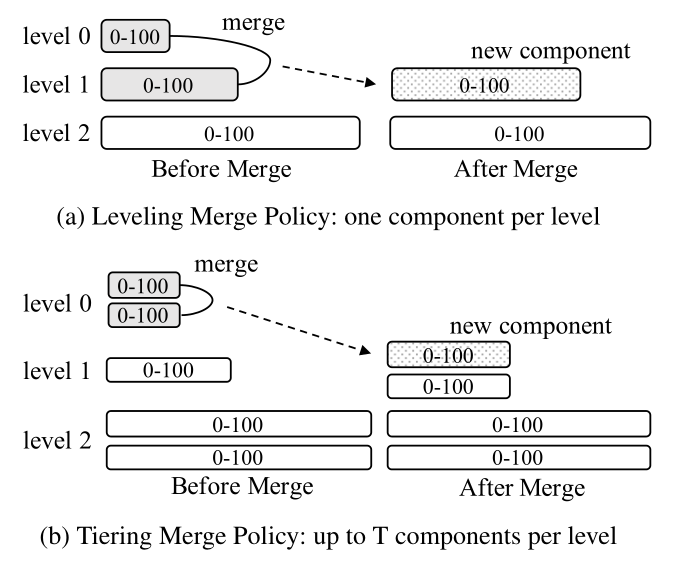
\includegraphics[width=.8\textwidth]{../../images/db/4.png}
\captionof{figure}{\label{}LSM-tree merge policies}
\end{center}
\begin{itemize}
\item \textbf{Leveling merge policy}: each level only maintains one component, but the component at level \(L\) is
\(T\) times larger than the component at level \(L-1\). As a result, the component at level \(L\)
will be merged multiple times with incoming component at level \(L-1\) until it fills up, and it
will then be merged into level \(L+1\), and it will then be merged into level \(L+1\).

\uline{Better query performance}.
\item \textbf{Tiering merge policy}: maintains up to \(T\) components per level. When level \(L\) is full, its
\(T\) components are merged together into a new component at level \(L+1\).

\uline{Better write performance}.
\end{itemize}
\subsection{Well-Known Optimizations}
\label{sec:orgf2e75c0}
\textbf{Bloom filter}:
\begin{itemize}
\item built on top of disk components.
\item built for each leaf page for a disk component: a point lookup can first search the non-leaf pages of
a \(B^+\)-tree to locate the leaf page, where the non-leaf pages are assumed to be small enough to
be cached, and then check the associated Bloom filter before fetching the leaf page.
\end{itemize}
The false positive rate of a Bloom filter is
\begin{equation*}
\left(1-e^{-kn}/m\right)^k
\end{equation*}
where \(k\) is the number of hash functions, \(n\) is the number of keys, and \(m\) is the total
number of bits. And the optimal number of hash functions that minimizes the false positive rate is
\begin{equation*}
k=\frac{m}{n}\ln 2
\end{equation*}
In practice, most systems typically use 10 bits/key as a default configuration, which gives a 1\% false
positive rate.

\textbf{Partitioning}: Partitioning is orthogonal to merge policies, both leveling and tiering can be adapted
to supported partitioning. But only the partitioned leveling policy has been fully implemented.

In the partitioned leveling merge policy, pioneered by LevelDB, the disk component at each level is
range partitioned into multiple fixed-size SSTables, as in figure \ref{lsm.4}
\begin{center}
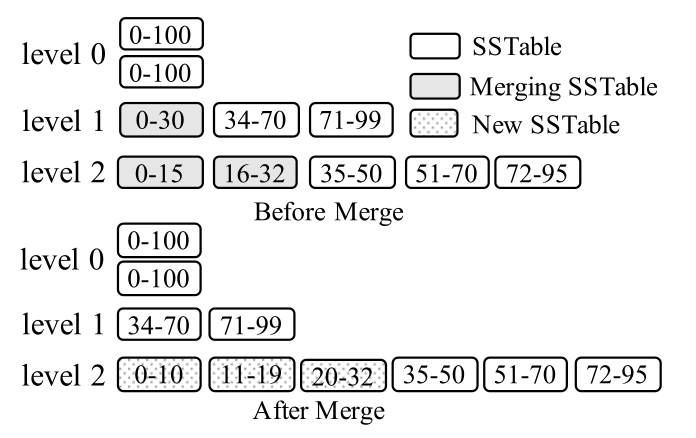
\includegraphics[width=.8\textwidth]{../../images/db/5.png}
\captionof{figure}{\label{lsm.4}Partitioned leveling merge policy}
\end{center}
Each SSTable is labeled with its key range in the figure. To merge an SSTable from level \(L\) into
level \(L+1\), all of its overlapping SSTable at level \(L+1\) are selected, and these SSTables are
merged with it to produce new SSTables still at level \(L+1\). Different policies can be used to
select which SSTable to merge next at each level.

The partitioned optimization can also be applied to the tiering merge policy. However, one major issue
in doing so is that each level can contain multiple SSTables with overlapping key ranges. Two possible
schemes can be used to organize the SSTables at each level
\begin{enumerate}
\item \textbf{Vertical grouping}: groups SSTables with overlapping key ranges together so that the groups have
disjoint key ranges
\item \textbf{Horizontal grouping}: each logical disk component, which is range-partitioned into a set of
SSTables, serves as a group directly
\end{enumerate}

\begin{center}
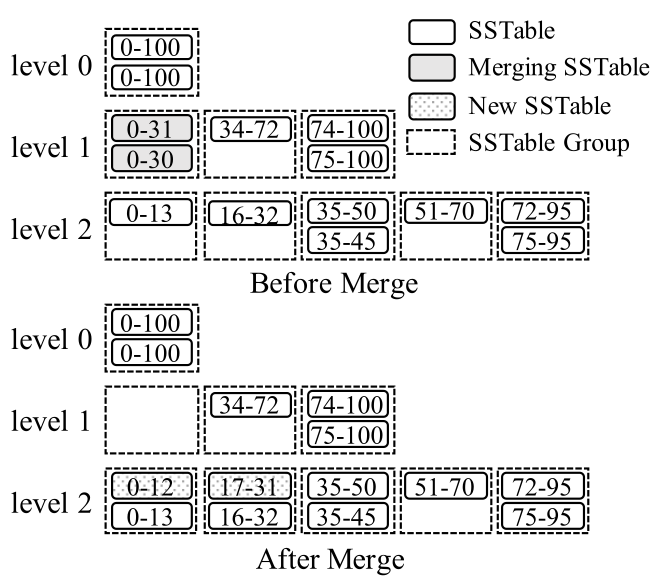
\includegraphics[width=.8\textwidth]{../../images/db/6.png}
\captionof{figure}{\label{}Partitioned tiering with vertical grouping}
\end{center}
During a merge operation, all of the SSTables in a group are merged together to produce the resulting
SSTables based on the key ranges of the overlapping groups at the next level, which are then added to
these overlapping groups.

\begin{center}
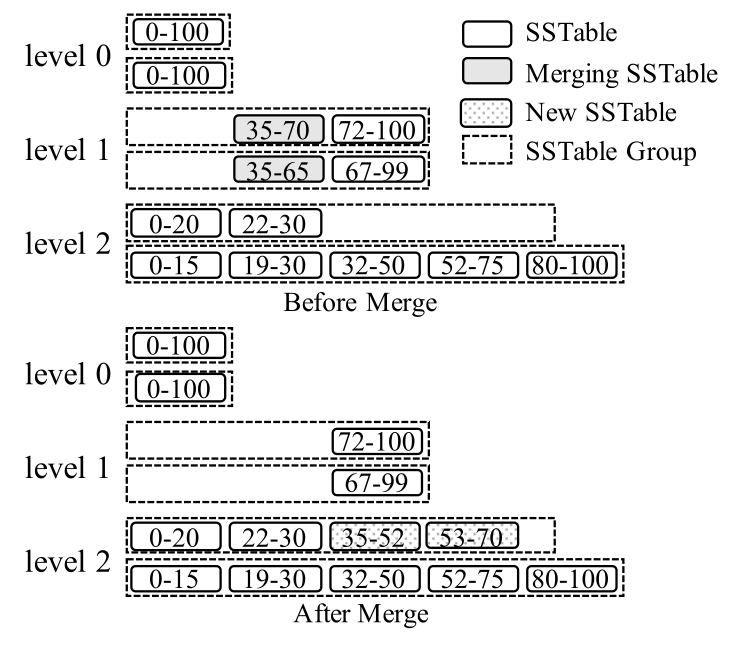
\includegraphics[width=.8\textwidth]{../../images/db/7.png}
\captionof{figure}{\label{}Partitioned tiering with horizontal grouping}
\end{center}
Each level \(L\) further maintains an active group, which is also the first group, to receive new
SSTables merged from the previous level. A merge operation selects the SSTables with overlapping key
ranges from all of the groups at a level, and the resulting SSTables are added to the active group at
the next level.
\subsection{Concurrency Control and Recovery}
\label{sec:org6839f06}
Depending on the transactional isolation requirement, today's LSM-tree implementations either use a
locking scheme or a multi-version scheme. A multi-version scheme works well with an LSM-tree since
obsolete can be \uline{garbage-collected} during merges.

Concurrent flush and merge operations, however, are unique to LSM-tree. These operations modify the
metadata of an LSM-tree, e.g., the list of active components. Thus, accesses to the component metadata
must be properly synchronized. To prevent a component in use from being deleted, each component can maintain a \uline{reference counter}.
Before accessing the components of an LSM-tree, a query can first obtain a snapshot of active
components and increment their in-use counters.

Since all writes are first appended into memory, write-ahead logging (WAL) can be performed to ensure
their durability. To simplify the recovery process, existing systems typically employ a \textbf{no-steal}
\textbf{buffer management policy}: a memory component can only be flushed when all active write transactions
have terminated. During recovery for an LSM-tree, the transaction log is replayed to redo all
successful transactions, but no undo is needed due to the no-steal policy.

Meanwhile, the list of active disk components must also be recovered in the event of a crash.
\begin{itemize}
\item For unpartitioned LSM-trees, this can be accomplished by \uline{adding a pair of timestamps of the stored
entries}.

This timestamp can be simply generated using local wall-clock time or a monotonic sequence number.
To reconstruct the component list, the recovery process can simply find all components with disjoint
timestamps. In the event that multiple components have overlapping timestamps, the component with
the largest timestamp range is chosen and the rest can simply be deleted since they will have been
merged to form the selected component.
\item For partitioned LSM-trees, a typical approach is to maintain a separate metadata log to store all
changes to the structural metadata, such as adding or deleting SSTables. The state of the LSM-tree
structure can then be reconstructed by replaying the metadata log during recovery.
\end{itemize}
\subsection{Cost Analysis}
\label{sec:org44c8a82}
\label{2.3}
The cost of writes and queries is measured by counting the number of disk I/Os per operation. This
analysis considers an unpartitioned LSM-tree and represents a worst-case cost.

Define
\begin{align*}
T&=\text{size ratio of a given LSM-tree}\\
L&=\text{levels of the LSM-tree}\\
B&=\text{number of entries that each data page can store, page size}\\
P&=\text{number of pages of a memory component}
\end{align*}

As a result, a memory component will contain at most \(B\cdot P\) entries., and level \(i\) will
contain at most \(T^{i+1}\cdot B\cdot P\) entries. Given \(N\) total entries, the largest level
contains approximately \(N\cdot\frac{T}{T+1}\). Thus the number of levels for \(N\) entries can be
approximated as \(L=\ceil{\log_T\left(\frac{N}{B\cdot P}\cdot\frac{T}{T+1}\right)}\)

The write cost, which is also referred to as \textbf{write amplification} in the literature, measures the
amortized I/O cost of inserting an entry into an LSM-tree. It should be noted that this cost measures
the overall I/O cost for this entry to be merged into the largest level since inserting an entry into
memory does not incur any disk I/O.
\begin{itemize}
\item For leveling, a component at each level will be merge \(T-1\) times until it fills up and is pushed
to the next level.
\item For tiering, multiple components at each level are merged only once and are pushed to the next level
directly.
\end{itemize}

Since each disk page contains \(B\) entries, the write cost for each entry will be
\(O(T\cdot\frac{L}{B})\) for leveling and \(O(\frac{L}{B})\) for tiering.

The I/O cost of a query depends on the number of components in an LSM-tree.
\begin{itemize}
\item Without Bloom filters, the I/O cost of a point lookup will be \(O(L)\) for leveling and
\(O(T\cdot L)\) for tiering.
\item For a zero-result point lookup, suppose all Bloom filters have \(M\) bits in total and have the same
false positive rate across all levels. With \(N\) total keys, each Bloom filter has a false positive
rate of \(O(e^{-\frac{M}{N}})\). Thus the I/O cost of a zero-result point lookup will be
\(O(L\cdot e^{-\frac{M}{N}})\) for leveling and \(O(T\cdot L\cdot e^{-\frac{M}{N}})\).
\item To search for an existing unique key, at least one I/O must be performed to fetch the entry. Given
that in practice the Bloom filter false positive rate is much smaller than 1, the successful point
lookup I/O cost for both the leveling and tiering will be \(O(1)\).
\end{itemize}

The I/O cost of a range query depends on the query selectivity. Let \(s\) be the number of unique keys
accessed by a range query. A range query can be considered to be \textbf{long} if \(\frac{s}{B}>2\cdot L\), and
\textbf{short} otherwise. The distinction is that the I/O cost of a long range query will be dominated by the
largest level since the largest level contains most of the data. In contrast, the I/O cost of a short
range query will derive equally from all levels since the query must issue one I/O to each disk
component. Thus, the I/O cost of a long range query will be \(O(\frac{s}{B})\) for leveling and
\(O(T\cdot\frac{s}{B})\) for tiering. For a short range query, the I/O cost will be \(O(L)\) for
leveling and \(O(T\cdot L)\) for tiering.

Finally, let's examine the space amplification of an LSM-tree, which is defined as the overall number
of entries divided by the number of unique entries.
\begin{itemize}
\item For leveling, the worst case occurs when all of the data at the first \(L-1\) levels, which contain
approximately \(\frac{1}{T}\) of the total data, are updates to the entries at the largest level.
Thus the worst case space amplification for leveling is \(O(\frac{T+1}{T})\).
\item For tiering, the worst case happens when all of the components at the largest level contain exactly
the same of keys. As a result, the worst case space amplification is \(O(T)\).
\end{itemize}

\begin{center}
\begin{tabular}{llllll}
Merge Policy & Write & Point Lookup (Zero-Result/Non-zero) & Short Range Query & Long Range Query & Space Amplification\\
Leveling & \(O(T\cdot\frac{L}{B})\)) & \(O(L\cdot e^{-\frac{M}{N}})/O(1)\) & \(O(L)\) & \(O(\frac{s}{B})\) & \(O(\frac{T+1}{T})\)\\
Tiering & \(O(\frac{L}{B})\) & \(O(T\cdot L\cdot e^{-\frac{M}{N}})/O(1)\) & \(O(T\cdot L)\) & \(O(T\cdot\frac{s}{B})\) & \(O(T)\)\\
\end{tabular}
\end{center}
\section{LSM-tree Improvements}
\label{sec:org390619f}
\subsection{A Taxonomy of LSM-tree Improvements}
\label{sec:org7439ddf}
\begin{itemize}
\item \textbf{Write Amplification}:
\item \textbf{Merge Operations}: Moreover, merge operations can have negative impacts on the system, including
buffer cache misses after merges and write stalls during large merges.
\item \textbf{Hardware}:
\item \textbf{Special Workloads}:
\item \textbf{Auto-Tuning}: Based on the RUM conjecture, no access method can be read-optimal, write-optimal, and
space- optimal at the same time.
\item \textbf{Secondary Indexing}:
\end{itemize}
\subsection{Reducing Write Amplification}
\label{sec:orge5c59d8}
\subsubsection{Tiering}
\label{sec:org580a848}
WriteBuffer (WB) tree:
\begin{enumerate}
\item hash-partitioning to achieve workload balance so that each SSTable group roughly stores the same
amount of data.
\item Organizes SSTable groups into a \(B^+\)-tree-like structure to enable self-balancing to minimize
the total number of levels. Specifically, each SSTable group is treated like a node in a
\(B^+\)-tree. When a non-leaf node becomes full with \(T\) SSTables, these \(T\) SSTables are
merged together to form a new SSTables that are added into its child nodes. When a leaf node
becomes full with \(T\) SSTables, it is split into two leaf nodes by merging all of its SSTables
into two leaf nodes with smaller key ranges so that each new node receives about \(T/2\) SSTables.
\end{enumerate}

The light-weight compaction tree presents a method to achieve workload balancing of SSTable groups.

dCompaction introduces the concept of virtual SSTables and virtual merges to reduce the merge
frequency. A virtual merge operation produces a virtual SSTable that simply points to the input
SSTables without performing actual merge. However, since a virtual SSTable points to multiple
SSTables with overlapping ranges, query performance will degrade. To address this, dCompaction
introduces a threshold based on the number of real SSTables to trigger actual merges. It also lets
queries trigger actual merges if a virtual SSTable pointing too many SSTables is encountered during
query processing.
\subsubsection{Merge Skipping}
\label{sec:org8b32ac1}
The skip-tree proposes a merge skipping idea to improve write performance. The observation is that
each entry must be merged from level 0 down to the largest level. If some entries can be directly
pushed to a higher level by skipping some level-by-level merges, then the total write cost will be
reduced.
\begin{center}
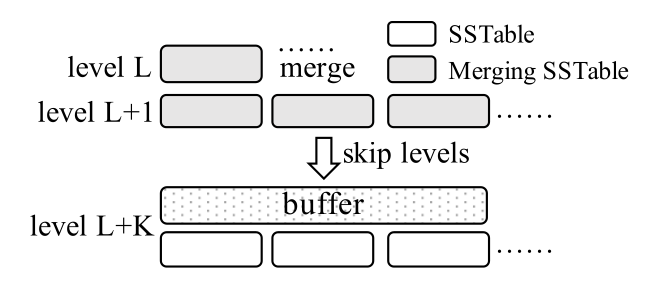
\includegraphics[width=.8\textwidth]{../../images/db/8.png}
\captionof{figure}{\label{}Merge in skip-tree}
\end{center}
During a merge at level \(L\), the skip-tree directly pushes some keys to a mutable buffer at level
\(L+K\) so that some level-by-level merges can be skipped. Meanwhile, the skipped entries in the
mutable buffer will be merged with the SSTables at level \(L+K\) during subsequent merges. To ensure
correctness, a key from level \(L\) can be pushed to level \(L+K\) only if this key doe not appear in
any of the intermediate levels \(L+1,\dots,L+K-1\). This condition can be tested efficiently by
checking the Bloom filters of the intermediate levels.
\subsubsection{Exploiting Data Skew}
\label{sec:org7e9719e}
TRIAD reduces write amplification for skewed update workloads where some hot keys are updated
frequently. The basic idea is to separate hot keys from cold keys in the memory component so that only
cold keys are flushed to disk. Even though hot keys are not flushed to disk, they are periodically
copied to a new transaction log so that the old transaction log can be reclaimed

TRIAD also reduces write amplification by delaying merges at level 0 until level 0 contains multiple
SSTables.

Finally, it presents an optimization that avoids creating new disk components after flushes. Instead,
the transaction log itself is used as a disk component and an index structure is built on top of it to
improve lookup performance.
\subsubsection{Summary}
\label{sec:org23ae03b}
Tiering has been widely used to improve the write performance of LSM-trees, but this will decrease
query performance and space utilization
\subsection{Optimizing Merge Operations}
\label{sec:orga9515aa}
\subsubsection{Improving Merge Performance}
\label{sec:orgfe528da}
The VT-tree presents a stitching operation to improve merge performance. The basic idea is that when
merging multiple SSTables, if the key range of a page from an input SSTable does not overlap the key
ranges of any pages from other SSTables, then this page can be simply pointed to by the resulting
SSTable without reading and copying.

But is has a number of drawbacks:
\begin{enumerate}
\item cause fragmentation since pages are no longer continuously stored: introduce a stitching threshold
\(K\) so that a stitching operation is triggered only when there are at least \(K\) continuous
pages from an input SSTable
\item Since the keys in stitched pages are not scanned during a merge operation, a Bloom filter cannot be
reproduced: use quotient filters since multiple quotient filters can be combined directly without
accessing the original keys.
\end{enumerate}

Or we could slightly merge the phases of merge\cite{6877309} .
\subsubsection{Reducing Buffer Cache Misses}
\label{sec:org2b812bf}
Merge operations can interfere with the caching behavior of a system. After a new component is
enabled, queries may experience a large number of buffer cache misses since the new component has not
been cached yet.

The Log-Structured buffered Merge tree:
\begin{center}
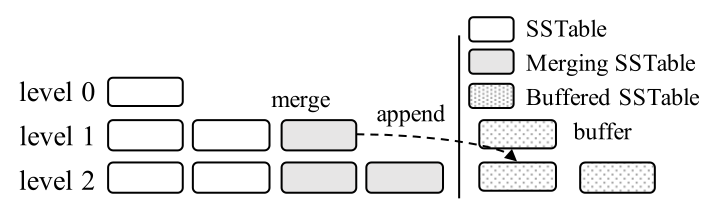
\includegraphics[width=.8\textwidth]{../../images/db/9.png}
\label{}
\end{center}
After an SSTable at level \(L\) is merged into level \(L+1\), the old SSTables at level \(L\) is
appended to a buffer associated with level \(L+1\) instead of being deleted immediately. The buffered
SSTables are searched by queries as well to minimize buffer cache misses, and they are deleted
gradually based on their access frequency. This approach is mainly effective for skewed workloads
where only a small range of keys are frequently accessed.
\subsubsection{Minimizing Write Stalls}
\label{sec:org2462c0f}
bLSM proposes a spring-and-gear merge scheduler to minimize write stalls for the unpartitioned
leveling merge policy. Its basic idea is to tolerate an extra component at each level so that merges
at different levels can proceed in parallel. Furthermore, the merge scheduler controls the progress of
merge operations to ensure that level \(L\)  produces a new component at level \(L+1\) only after the
previous merge operation at level \(L+1\) has completed.

bLSM was only designed for the unpartitioned leveling merge policy. Moreover, it only bounds the
maximum latency of writing to memory components while the queuing latency, which is often a major
source of performance variability, is ignored.
\subsubsection{Summary}
\label{sec:org3cee1a6}
\subsection{Hardware Opportunities}
\label{sec:org80b7899}
\subsubsection{Large Memory}
\label{sec:org5a9d2df}
\begin{itemize}
\item If a memory component is implemented directly using on-heap data structures, large memory can result
in a large number of small objects that lead to significant GC overheads.
\item If a memory component is implemented using off-heap structures such as a concurrent \(B^+\)-tree,
large memory can still cause a higher search cost (due to tree height) and cause more CPU cache
misses for writes, as a write must first search for its position in the structure.
\end{itemize}

Memory component scales badly. Image from FloDB's \href{https://pdfs.semanticscholar.org/ad61/262bd300e6e645b1a97bc657309e3f56df2c.pdf}{presentation}.
\begin{center}
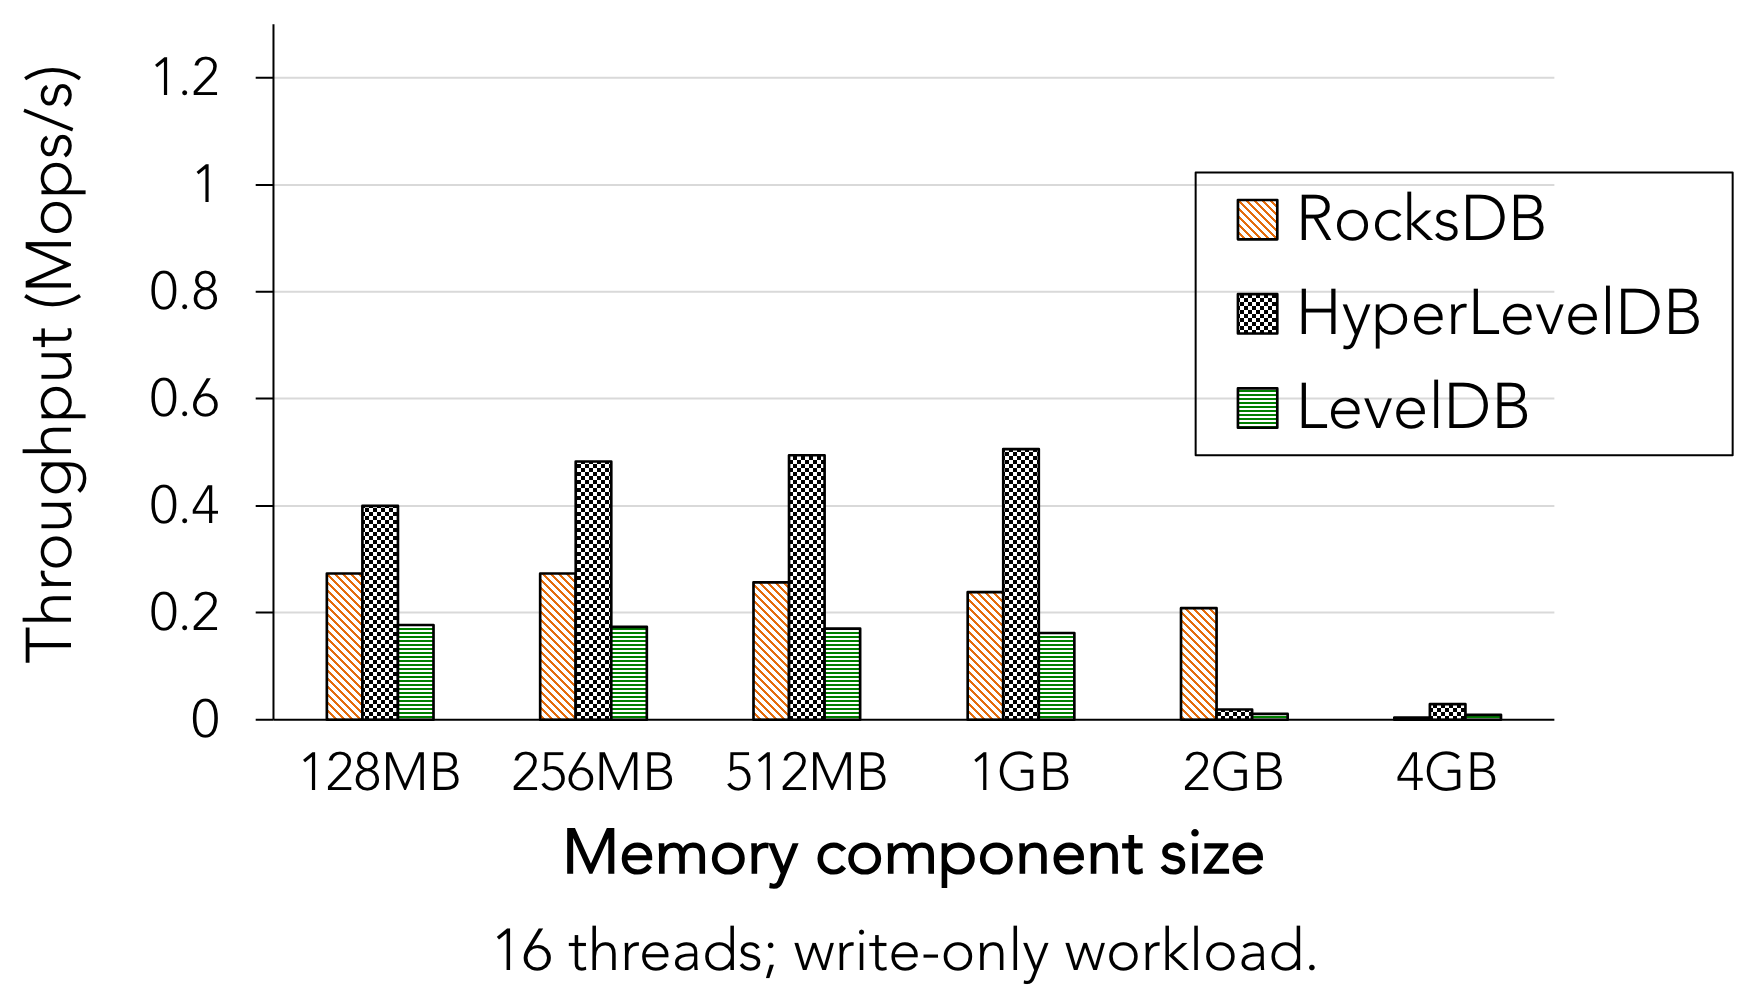
\includegraphics[width=.8\textwidth]{../../images/db/10.png}
\label{}
\end{center}

FloDB presents a two-layer design to manage large memory components.
\begin{itemize}
\item The top level is a small concurrent hash table to support fast writes, and the bottom level is a
large skip-list to support range queries efficiently.
\item When the hash table is full, its entries are efficiently migrated into the skip-list using a batched
algorithm.
\end{itemize}
By limiting random writes to a small memory area, this design significantly improves the in-memory
write throughput. To support range queries, FloDB requires that a range query must wait for the hash
table to be drained so that the skip-list alone can be searched to answer the query.

Problems:
\begin{enumerate}
\item Not efficient for workloads containing both writes and range queries.
\item The skip-list may have a large memory footprint and lead to lower memory utilization.
\end{enumerate}

To address the drawbacks of FloDB, Accordion uses a multi-layer approach to manage its large memory
components. In this design,
\begin{center}
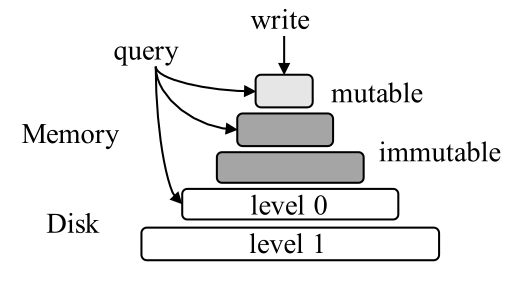
\includegraphics[width=.8\textwidth]{../../images/db/11.png}
\captionof{figure}{\label{}Accordion's multi-layer structure}
\end{center}
there is a small mutable memory component in the top level to process writes. When the mutable
component is full, instead of being flushed to disk, it is simply flushed into a immutable memory
component via an in-memory flush operation. Similarly, such immutable memory components can be merged
via in-memory merge operations to improve query performance and reclaim space occupied by obsolete entries.
\subsubsection{Multi-Core}
\label{sec:org7684a76}
cLSM\cite{10.1145/2741948.2741973} optimized for multi-core machines and presents new concurrency control algorithms for various
LSM-tree operations. It organizes LSM components into a concurrent linked list to minimize blocking
caused by synchronization. Flush and merge operations are carefully designed so that they only result
in atomic modifications to the linked list that will never block queries. When a memory component
becomes full, a new memory component is allocated while the old one will be flushed.
\subsubsection{SSD/NVM}
\label{sec:org9322926}
The FD-tree uses a similar design to LSM-trees to reduce random writes on SSDs. One major difference
is that the FD-tree exploits \textbf{fractional cascading}\cite{10.1007/BF01840440} to improve query performance
instead of Bloom filters.
For the component at each level, the FD-tree additionally stores fence pointers at each level. For
example,
\begin{center}
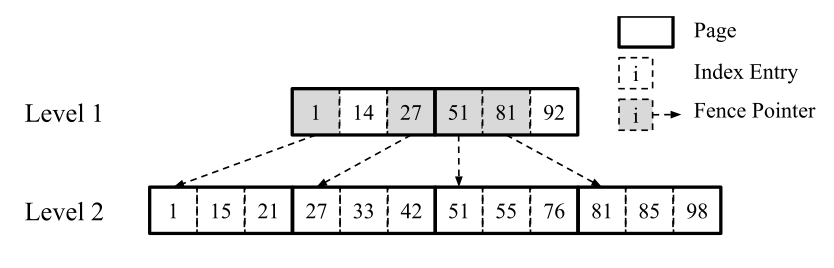
\includegraphics[width=.8\textwidth]{../../images/db/12.png}
\captionof{figure}{\label{}Example of FD-tree}
\end{center}
the pages at level 2 are pointed at by are pointed by fence pointers with keys 1, 27, 51, 81 at
level 1. After performing a binary search at level 0, a query can follow these fence pointers to
traverse all of the levels.

However, when the component at level \(L\) is merged into level \(L+1\), all of the previous levels 0
to \(L-1\) must be merged as well to rebuild the fence pointers.

The FD+tree improves the merge process of the FD-tree.

MaSM(materialized sort-merge) is designed for supporting efficient updates for data warehousing
workloads by exploiting SSDs. MaSM first buffers all updates into an SSD. It uses the tiering policy
to merge intermediate components with low write amplification. The updates are then merged back to the
base data.

Since SSDs support efficient random reads, separating values from keys becomes a viable solution to
improve the write performance of LSM-trees. This approach was first implemented by WiscKey and
subsequently adopted by HashKV and SifrDB. WiscKey stores key-value pairs into an append-only log and
the LSM-tree simply serves as a primary index that maps each key to its location in the log.

\begin{center}
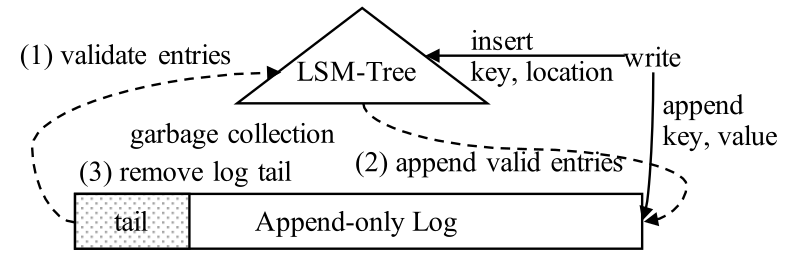
\includegraphics[width=.8\textwidth]{../../images/db/13.png}
\captionof{figure}{\label{}WIscKey stores values into an append-only log to reduce the write amplification}
\end{center}
As shown in Figure, WIscKey stores key-value pairs into an append-only log and the LSM-tree simply
serves as a primary index that maps each key to its location in the log. While this can greatly reduce
the write cost by only merging keys, range query will be significantly impacted. Moreover, the value
log must be garbage-collected efficiently to reclaim the storage space.

In WiscKey, garbage-collection is performed in three steps:
\begin{enumerate}
\item scan the log tail and validates each entry by performing point lookups against the LSM-tree to find
out whether the location of each key has changed or not.
\item Valid entries, whose locations haven't changed, are then appended to the log their locations are
updated in the LSM-tree as well
\item log tail is truncated to reclaim the storage space.
\end{enumerate}

HashKV introduces a more efficient approach to garbage-collect obsolete values. The basic idea is to
hash-partition the value log into multiple partitions based on keys and to garbage-collect each
partition independently. In order to garbage-collect a partition, HashKV performs a group-by operation
on the keys to find the latest value for each key. Valid key-value pairs are added to a new log and
their locations are then updated in the LSM-tree. HashKV further stores cold entries separately so
that they can be garbage-collected less frequently.

NoveLSM is an implementation of LSM-trees on NVMs.
\subsubsection{Native Storage}
\label{sec:orge59843d}
\subsection{Handling Special Workloads}
\label{sec:orgeb124bb}
temporal data, small data, semi-sorted data, append-mostly data.
\subsection{Auto-Tuning}
\label{sec:org62ace6c}
\subsubsection{Parameter Tuning}
\label{sec:org29dcaba}
\cite{10.5555/2930583.2930595}  presented an analytical model that incorporates the key distribution to
improve the cost estimation of LSM-tree operations and further used this model to tune the parameters
of LSM-trees. If a key is found to be deleted or updated during an early merge, it will not
participate in future merges and thus its overall write cost will be reduced. The proposed model
assumes a priori knowledge of the key distribution using a probability mass function \(f_X(k)\) that
measures the probability that a specific key \(k\) is written by a write request. Given \(p\) total
write requests, the number of unique keys is estimated using its expection as
\(Unique(p)=N-\sum_{k\in K}(1-f_X(k))^p\), where \(N\) is the total number of unique keys and \(K\) is
the total key space.

Monkey co-tunes the merge policy, size ratio, and memory allocation between memory components and
Bloom filters to find an optimal LSM-tree design for a given workload.

Monkey shows that the usual Bloom filter memory allocation scheme, which allocates the same number
of bits per key for all Bloom filters, results in sub-optimal performance: the intuition is that
the \(T\) components at the last level, which contain most of the data, consume most of the Bloom
filter memory but their Bloom filters can only save at most \(T\) disk I/Os for a point lookup. To
minimize the overall false positive rates across all of the Bloom filters, Monkey analytically
shows that more bits should be allocated to the components at the lower level, and the new I/O
becomes \(O(e^{-\frac{M}{N}})\) for leveling and \(O(T\cdot e^{-\frac{M}{N}})\) for tiering. Monkey
then finds an optimal LSM-tree design by maximizing the overall throughput using a cost model similar
to the one in \ref{2.3}.
\subsubsection{Tuning Merge Policies}
\label{sec:org7599398}
For leveling, the cost of zero-result point lookups, long range queries, and space amplification are
dominated by the largest level, but the write cost derives equally from all of the levels. To address
this, Dostoevsky\cite{10.1145/3183713.3196927} introduces a lazy-leveling merge policy that performs
tiering at the lower levels but leveling at the largest level.

Lazy-leveling has much better write cost than leveling, but has similar point lookup cost, long range
query cost, and space amplification to leveling. It only has a worse short range query cost than
leveling.
\subsubsection{Dynamic Bloom Filter Memory Allocation}
\label{sec:org831ebde}
ElasticBF dynamically adjusts the Bloom filter false positive rates based on the data hotness and
access frequency to optimize read performance. Given a budget of \(k\) Bloom filter bits per key,
ElasticBF constructs multiple smaller Bloom filters with \(k_1,\dots,k_n\) bits so that
\(k_1+\dots+k_n=k\). When all of these Bloom filters are used together, they provide the same false
positive rate as the original monolithic Bloom filter. ElasticBF then dynamically activates and
deactivates these Bloom filters based on the access frequency to minimize the total amount of extra
I/O. Their experiments reveal that ElasticBF is mainly effective when the overall Bloom filter memory is very limited.
\subsubsection{Optimizing Data Placement}
\label{sec:org694bb06}
For cloud
\subsection{Secondary Indexing}
\label{sec:orgb70854c}
In general, an LSM-based storage system will contain a primary index with multiple secondary indexes.
The primary index stores the record values indexed by their primary keys. Each Secondary index stores
the corresponding primary keys for each secondary key using either a composite key approach or a key
list approach:
\begin{itemize}
\item In the composite key approach, the index key of a secondary index is the composition of the
secondary key and the primary key.
\item In the key list approach, a secondary index associates a list
\end{itemize}
of primary keys with each secondary key.

Either way, to process a query using a secondary index, the secondary index is first searched to
return a list of matching primary keys, and those are then used to fetch the records from the primary
index if needed. For example:
\begin{center}
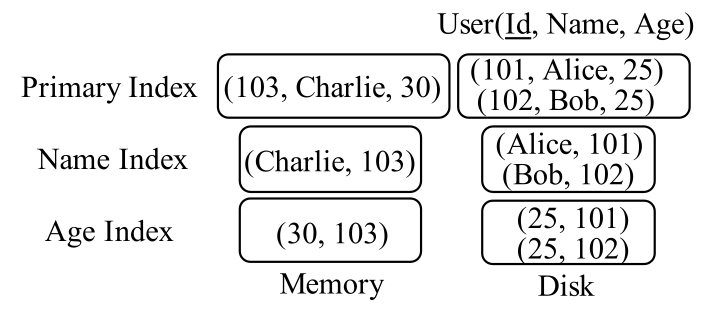
\includegraphics[width=.8\textwidth]{../../images/db/14.png}
\captionof{figure}{\label{}Example LSM-based secondary indexes}
\end{center}
\subsubsection{Index Structures}
\label{sec:org59f1200}
\subsubsection{Index Maintenance}
\label{sec:org0cd6200}
\section{{\bfseries\sffamily TODO} Papers that worth read [0/0]}
\label{sec:orgbfd7d73}
\begin{itemize}
\item[{$\square$}] Monkey
\end{itemize}
\section{References}
\label{sec:org17833f1}
\label{bibliographystyle link}
\bibliographystyle{alpha}

\label{bibliography link}
\bibliography{../../references}
\end{document}
